\section{Experience}

Key ideas:

\begin{itemize}
	\item Data Elements can be used across different DataModels - favourites or shopping cart.
	\item Unique Identification of DataElements 
	\item Documentation can be automatically generated for review purposes
	\item Consistency checking carried out on data elements
	\item Generation of XSDs, XML, and Forms as output, interfacing with OpenClinica.
	\item Data Provenance
\end{itemize}


\subsection{NHIC}

The NIHR-funded HIC project is concerned with the creation of research
datasets in five key clinical domains: Acute Coronary Syndromes,
Hepatology, Intensive Care, Ovarian Cancer, and Renal Transplantation.
Each is to populated with data taken from routine clinical care, and
integrated across five of the largest teaching hospitals in the United
Kingdom.

This project provided a number of challenges:

\begin{itemize}
\item To define an appropriate dataset for each of the five themes
  that could be re-used in future research studies, and linked to
  external data sources.
\item To understand and clarify the differences in data collection
  across the five sites, and record this in a suitable manner for
  researchers to review at a later date.
\item To define common data collection tools, such that each site
  could collate and submit their own data to the lead site.

\end{itemize}

In each theme, the process of data-modelling started with the
identification of key data points that are recognised as important for
all research in that domain.  For example in Cancer treatment, the
size and shape of any tumour before and after any intervention are
important.  This process was primarily carried out by domain-experts -
the academic clinicians with a knowledge of the data required for
research, and the data collected during core clinical care.  Also
involved in the process were nurses responsible for collecting the
data in routine care of clinical trials, the researchers involved in
disseminating data in trials, and the IT staff charged with storing
and collating data, who understand what may be available.

Most of this initial modeling was carried out via Excel spreadsheets:
many existing datasets are defined in this form and so was familiar to
the domain experts.  We built an importer for the model catalogue that
allowed these Excel spreadsheets to be parsed and stored according to
the Model Catalogue schema.  We recorded links between datapoints in
the HIC datasets and those in pre-existing reporting datasets.  In
some cases these were auto-detected, in some cases recorded manually
through the model catalogue interface, and in some cases these were
imported via the Excel documents.  

In each theme, existing datasets had already been defined, with the
purpose of providing summary data for hospitals charging services, or
for national reporting against predefined targets.  In many cases
these data points were a good starting point for a research dataset,
but data collected was not sufficiently granular, or additional
data points were required for the purposes of clinical research.

For each data point, the sites recorded how that data was collected.
In the simplest case, that would include the value domain, and any
constraints on allowable values imposed by the collection tool.  It
became apparent that different sites may collect the same data point
according to different enumerated domains.  Where these values were
later submitted as part of, for example, a national reporting dataset,
these values would be translated, often resulting in a loss of
fidelity.  

It was clear that such transformations, and unification across a
number of different sites led to a great loss in information; each
data point being reduced to a lowest-common denominator.  One of the
key principles of the HIC programme was that each site should submit
data in the way in which it was collected, and document in the model
catalogue the way in which it was recorded.


In conjunction with this process, an exercise was undertaken at each
site to audit the quality, coverage, and consistency of the data at
each data point.  This helped to inform a pragmatic set of data which
might prove to be valuable in the short-term.

Each theme then refined the datasets into a number of structured
models.  In the first instance, UML class diagrams were created,
showing grouping and multiplicities of data.  For example,
measurements corresponding to the size and shape of a tumour may be
grouped according to the particular tumour that is of interest.  A
patient may have a number of tumours, and for each tumour, the size
and shape may be mandatory fields.

Where appropriate, patient pathway models were created to add
additional context.  Similar to a workflow diagram, the patient
pathway models described the common routes through the care system
that a patient may take.  Each data point was associated with one or
more points on the diagram, indicating where each data point is
collected, and where it may be used later on in making a decision
about the particular treatment a patient is to receive.

These models were typically created by the technical team in
collaboration with the domain experts.  In many cases, the patient
pathways were more complex than the clinicians had realised - and the
process of creating the models helped both parties understand the
complexity of the domain.  The models are preserved in the catalogue
for future re-use.

In most cases, these models served as a general purpose description
for each clinical theme.  However, differences in treatment at
different sites often led to distinctions being made: different models
were required for different sites.  For example, the decision whether
a particular cancer patient would be treated with surgery or
chemotherapy may be made differently at different sites, thus changing
the meaning of any data subsequently collected about that patient.

For each theme, we generated an XML schema, allowing each site to
submit their data according to a common structure.   


\subsection{Genomics England - reuse of HIC Models}

One of the prime tasks of Genomics England (GEL) is to integrate a patient's clinical records with that patients genome, and use this integrated data to inform new clinical research primarily in the domain of genetic medicine. In order to do this GEL is assembling core datamodels, initially to classify clinical research in the area of rare diseases and in the area of cancer.  In order to do this clinicians were asked to assemble datamodels in excel and XML format, and attempt to arrive at an agreed datamodel for the two areas.  Initially this was carried out by assembling the subject matter experts in a conference room and then going through each item in turn. The process was quite time consuming and difficult, mostly because the users were mostly eminent clinicians and extremely busy, so that getting all the contributors in the same room at the same time was itself quite a difficult task to achieve.

Whilst that process was being carried out, some of these datasets were added to the Model Catalogue, and the subject matter experts were given visibility of the datasets already stored in the Model Catalogue. At this point the Model Catalogue was already loaded with datasets derived from the NHS Data disctionary such as COSD and from the results of the NHIC work. Use of the toolkut resulted in the users being able to very quickly assemble a new dataset from an existing dataset; they were then able to go through each data element in turn and compare it to an existing data element in another datamodel, a process that is illustrated in figure \ref{fig:dataClassComparison}.

For the Genomics England exercise the Models Catalogue has been had an added social networking feature added, allowing messaging forums to be automatically generated around a \emph{datamodel} or \emph{dataclass} . This allows users to develop a new draft datamodel, and then 

From looking at the datasets we can see that in the first 2 major datamodels produced X\% of data elements and dataclasses were derived from existing sources, a fact entirely due to the use of the Model Catalogue in the data curation process. Time to assemble a new datamodel has been cut from months to weeks as a result of having a single shared source for the datamodel, and having the means to electronically comment on and discuss datamodel development in real time as it is happening.



 Figure \ref{fig:dataClassComparison}
 \begin{figure}[here]
 	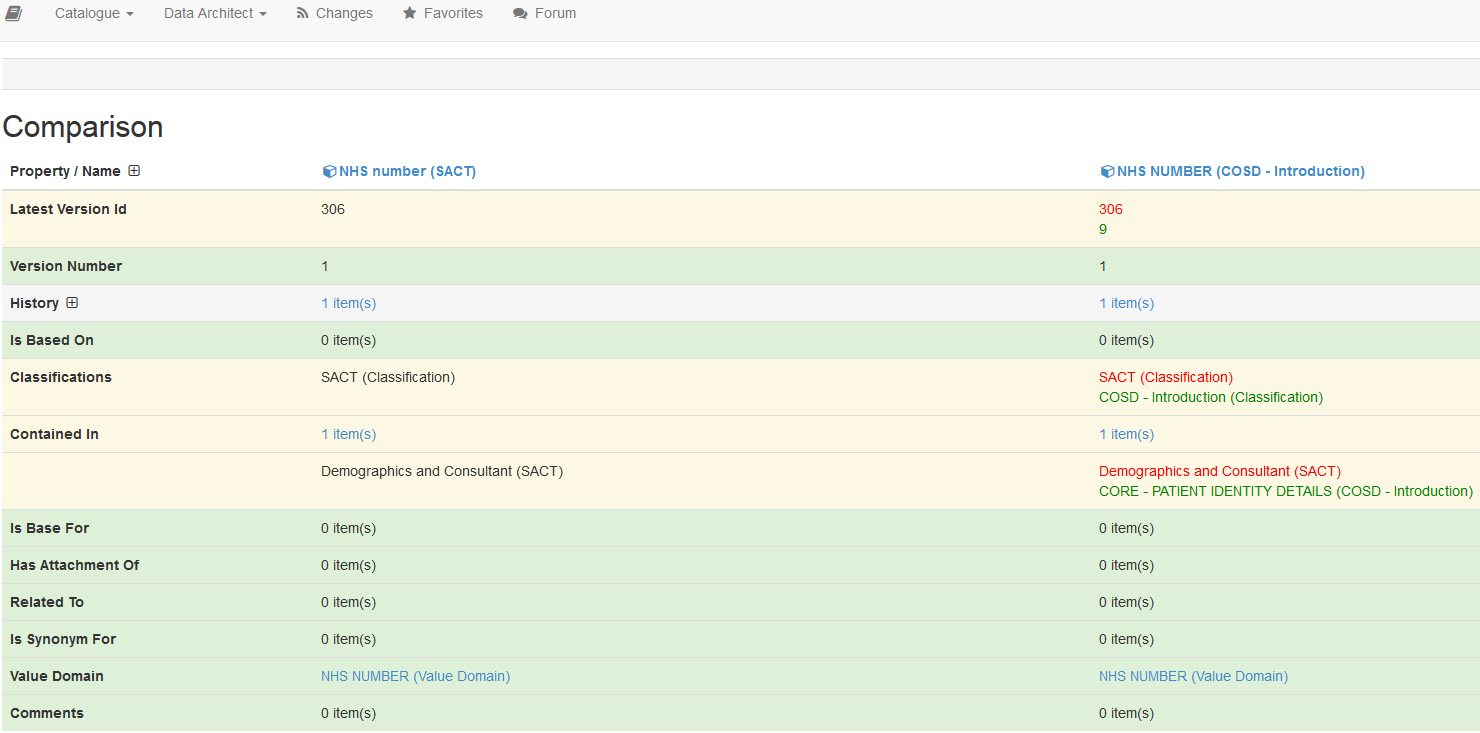
\includegraphics[width=0.5\textwidth,natwidth=610,natheight=642]{ComparisonOfDataClasses}
 	\caption{Screen Shot of DataClass Comparison} 
 	\label{fig:dataClassComparison}	
 \end{figure}



\subsection{Genomics England -  deployment}
